\begin{frame}[fragile]{Tracking: The Four File Status}
  \begin{figure}
    \caption{The lifecycle of the status of your files}
    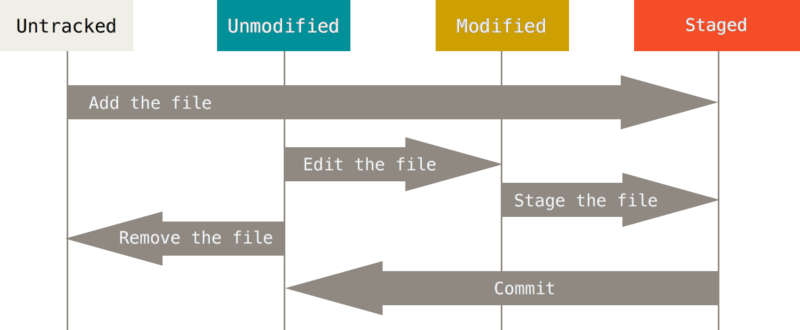
\includegraphics[width=\textwidth]{tracking/lifecycle}
  \end{figure}
  \begin{columns}[t]
    \begin{column}{0.5\textwidth}
      \footnotesize
In a repository, a file can exist in one of four status: Untracked, Unmodified,
Modified, or Staged.
    \end{column}
    \begin{column}{0.5\textwidth}
      \footnotesize
      The main tool you use to determine which files are in which status is:
        \begin{minted}[
            breaklines,
            frame=single,
            fontsize=\footnotesize
          ]{bash}
git status
        \end{minted}
    \end{column}
  \end{columns}
\end{frame}
